% !TEX root = main.tex
\section{Nueva función Wilbur \label{sec:other_wilbur_func}}

Se adopta una nueva función Wilbur para la versión 1.0 de Nebulas NOVA.

\begin{align}
\label{al:new_wilbur}
f(x) = x/(1 + (\frac{a}{x})^b) \quad a>0,0<b<1
\end{align}

\begin{figure}
\centering
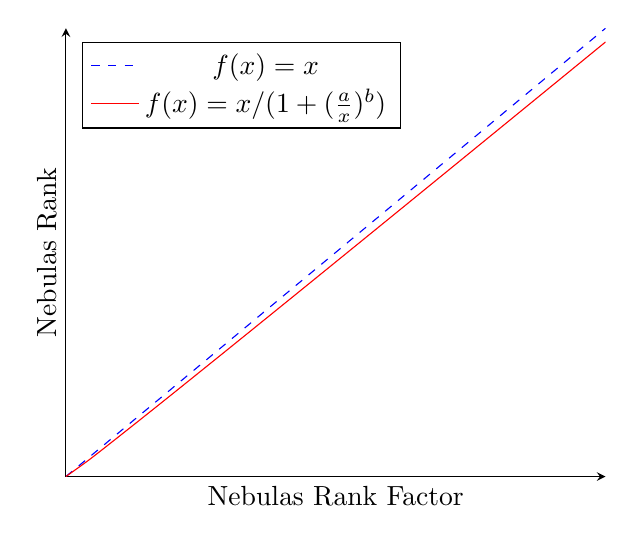
\begin{tikzpicture}[
    declare function={func(\x,\mu) = (\x / (1 + (1/\x)^(0.5)));},
    declare function={linefunc(\x) = \x;}
]
\begin{axis}[
    axis lines=left,
    enlargelimits=upper,
ticks=none,axis x line=bottom,axis y line=left,xlabel={Nebulas Rank Factor},
  ylabel={Nebulas Rank},
      legend pos=north west,
legend style={fill=none}
]
\addplot [dashed, domain=0:1000, blue] {linefunc(x)};
\addplot [smooth, domain=0:1000, red] {func(x,3)};
\addlegendentry{$f(x)=x$}
\addlegendentry{$f(x) = x/(1 + (\frac{a}{x})^b)$}
\end{axis}
\end{tikzpicture}
\caption{Curva de la función de Nebulas Rank}
\label{fig:new_wilbur}
\end{figure}

Como se muestra en la figura \ref{fig:new_wilbur}, es sencillo demostrar que la función satisface las dos propiedades \ref{prop:one}, \ref{prop:two} y en \refsec{sec:function}.